\chapter{Desarrollo}

\section{Integraci\'on con ThreeJs}
La soluci\'on elegida para extender el sistema de materiales de Three ha sido crear un fork, extendiendo la
librer\'ia para implementar las funcionalidades necesarias que dan soporte a estos nuevos motores de shading.
Siguiendo la nomenclatura, de ThreeJs (MeshStandardMaterial, MeshPhysicalMaeterial, etc) se ha creado un material
MeshClothMaterial, basado en los material Cloth de Filament.\\
ThreeJS utiliza un sistema de chunks (trozos) se componen en tiempo de ejecuci\'on para acabar formando los vertex
y fragment shaders que se utilizan en los programas de WebGL. Los chunks se componen en la libreria de shaders, la
clase ShaderLib.
Para crear nuestro MeshClothMaterial, hemos de extender de la clase base Material, de la que extienden el resto de
materiales. En este caso, de la misma forma que hace MeshPhysicalMaterial, extenderemos de MeshStandardMaterial,
que dispone de la mayor parte de uniforms y attributes que necesita nuestro shader.\\

\bgroup
  \begin{lstlisting}[caption=Clase MeshClothMaterial]
    import { Vector2 } from '../math/Vector2.js';
    import { MeshStandardMaterial } from './MeshStandardMaterial.js';
    import { Color } from '../math/Color.js';
    import brdfCloth from './clothBRDF.js';
    
    /**
     * parameters = {
     *  reflectivity: <float>,
     *
     *  sheen: <Color>,
     *
     *  transmission: <float>,
     *  transmissionMap: new THREE.Texture( <Image> ),
     *
     *  subsurface: <Vector3>,
     * }
     */
    
    function MeshClothMaterial( parameters ) {
    
      MeshStandardMaterial.call( this );
    
      this.defines = {
    
        'STANDARD': '',
        'CLOTH': ''
    
      };
    
      this.type = 'MeshClothMaterial';
      this.sheen = null;
    
      this.transmission = 0.0;
      this.transmissionMap = null;
      this.subsurface = null;
    
      this.brdfCloth = brdfCloth;
    
      this.setValues( parameters );
    
    }
    
    MeshClothMaterial.prototype = Object.create( MeshStandardMaterial.prototype );
    MeshClothMaterial.prototype.constructor = MeshClothMaterial;
    
    MeshClothMaterial.prototype.isMeshClothMaterial = true;
    
    MeshClothMaterial.prototype.copy = function ( source ) {
    
      MeshStandardMaterial.prototype.copy.call( this, source );
    
      this.defines = {
    
        'STANDARD': '',
        'CLOTH': ''
    
      };
    
      if ( source.sheen ) {
    
        this.sheen = ( this.sheen || new Color() ).copy( source.sheen );
    
      }
    
      this.transmission = source.transmission;
      this.transmissionMap = source.transmissionMap;
    
      if ( source.subsurface ) {
    
        this.subsurface = ( this.subsurface || new Color() ).copy( source.subsurface );
    
      } else {
    
        this.subsurface = null;
    
      }
    
      if ( source.brdfCloth ) {
    
        this.brdfCloth = source.brdfCloth;
    
      } else {
    
        this.brdfCloth = null;
    
      }
    
      return this;
    
    };
    
    export { MeshClothMaterial };
    
  \end{lstlisting}
  
  Para que el motor de render de ThreeJS reconozca este nuevo material es necesario, a\~nadir
  su tipo (MeshClothMaterial) al mapa de ShaderIds para que el gestor de programas (WebGLPrograms)
  lo utilice para detectar obtener los uniforms y shaders necesarios para el material. Adem\'as
  los nuevos par\'ametros necesarios para el material se deben de incluir en el array
  parametersNames, de forma que el sistema de cacheo de programas de ThreeJS detecte estas
  nuevas propiedades.\newline
  
  \begin{lstlisting}[caption=Clase MeshClothMaterial]
  function WebGLPrograms( renderer, cubemaps, extensions, capabilities, bindingStates, clipping ) {
  
    // ...
  
    const shaderIDs = {
      MeshDepthMaterial: 'depth',
      MeshDistanceMaterial: 'distanceRGBA',
      MeshNormalMaterial: 'normal',
      MeshBasicMaterial: 'basic',
      MeshLambertMaterial: 'lambert',
      MeshPhongMaterial: 'phong',
      MeshToonMaterial: 'toon',
      MeshStandardMaterial: 'physical',
      MeshPhysicalMaterial: 'physical',
      MeshClothMaterial: 'cloth',
      MeshMatcapMaterial: 'matcap',
      LineBasicMaterial: 'basic',
      LineDashedMaterial: 'dashed',
      PointsMaterial: 'points',
      ShadowMaterial: 'shadow',
      SpriteMaterial: 'sprite'
    };
  
    const parameterNames = [
      "precision", "isWebGL2", "supportsVertexTextures", "outputEncoding", "instancing", "instancingColor",
      "map", "mapEncoding", "matcap", "matcapEncoding", "envMap", "envMapMode", "envMapEncoding", "envMapCubeUV",
      "lightMap", "lightMapEncoding", "aoMap", "emissiveMap", "emissiveMapEncoding", "bumpMap", "normalMap", "objectSpaceNormalMap", "tangentSpaceNormalMap", "clearcoatMap", "clearcoatRoughnessMap", "clearcoatNormalMap", "displacementMap", "specularMap", "subsurface", "brdfCloth",
      "roughnessMap", "metalnessMap", "gradientMap",
      "alphaMap", "combine", "vertexColors", "vertexTangents", "vertexUvs", "uvsVertexOnly", "fog", "useFog", "fogExp2",
      "flatShading", "sizeAttenuation", "logarithmicDepthBuffer", "skinning",
      "maxBones", "useVertexTexture", "morphTargets", "morphNormals",
      "maxMorphTargets", "maxMorphNormals", "premultipliedAlpha",
      "numDirLights", "numPointLights", "numSpotLights", "numHemiLights", "numRectAreaLights",
      "numDirLightShadows", "numPointLightShadows", "numSpotLightShadows",
      "shadowMapEnabled", "shadowMapType", "toneMapping", 'physicallyCorrectLights',
      "alphaTest", "doubleSided", "flipSided", "numClippingPlanes", "numClipIntersection", "depthPacking", "dithering",
      "sheen", "transmissionMap"
    ];
  
    // ...
  
    function getParameters( material, lights, shadows, scene, object ) {
  
      const shaderID = shaderIDs[ material.type ];
  
      // ...
  
      let vertexShader, fragmentShader;
  
      if ( shaderID ) {
  
        const shader = ShaderLib[ shaderID ];
  
        vertexShader = shader.vertexShader;
        fragmentShader = shader.fragmentShader;
  
      }
  
      // ...
  
      const parameters = {
  
        shaderID: shaderID,
  
        vertexShader: vertexShader,
        fragmentShader: fragmentShader,
  
        sheen: !! material.sheen,
  
        subsurface: !! material.subsurface,
  
        brdfCloth: !! envMap && shaderID === 'MeshClothMaterial',
        // ...
      };
  
      // ...
  
      return parameters;
    }
  \end{lstlisting}
  
  Finalmente, en el gestor de materiales de ThreeJs, necesitamos a\~nadir un nuevo m\'etodo
  que actualice los unfiroms del programa creado, de la misma forma que se hace con los
  materiales nativos de la librer\'ia.\newline
  
  \begin{lstlisting}[caption=Clase WebGLMaterials]
  function refreshMaterialUniforms( uniforms, material, pixelRatio, height ) {
  
  // ...
  
  if ( material.isMeshStandardMaterial ) {
  
    refreshUniformsCommon( uniforms, material );
  
    if ( material.isMeshPhysicalMaterial ) {
  
      refreshUniformsPhysical( uniforms, material );
  
    } else if ( material.isMeshClothMaterial ) {
  
      refreshUniformsCloth( uniforms, material );
  
    } else {
  
      refreshUniformsStandard( uniforms, material );
  
    }
  
  }
  
  // ...
  
  function refreshUniformsCloth( uniforms, material, environment ) {
  
    refreshUniformsStandard( uniforms, material, environment );
  
    uniforms.reflectivity.value = material.reflectivity; // also part of uniforms common
  
    if ( material.sheen ) {
  
      uniforms.sheen.value.copy( material.sheen );
  
    } else {
  
      uniforms.sheen.value.copy( material.color );
      uniforms.sheen.value.r = Math.sqrt( uniforms.sheen.value.r );
      uniforms.sheen.value.g = Math.sqrt( uniforms.sheen.value.g );
      uniforms.sheen.value.b = Math.sqrt( uniforms.sheen.value.b );
  
    }
  
    if ( material.subsurface ) uniforms.subsurface.value.copy( material.subsurface );
  
    if ( material.brdfCloth ) uniforms.brdfCloth.value = material.brdfCloth;
  
  }
    
  \end{lstlisting}
  
  De esta forma, tenemos un material con la interfaz nativa de ThreeJS, que tiene acceso a los
  chunks definidos en la clase ShaderChunk y cuyos uniforms y composici\'on de chunks definiremos
  en ShaderLib.\newline
  
  El BRDF para el componente especular de la iluminaci\'on directa del material Cloth de Filament,
  se utiliza en ThreeJS para a\~nadir opcionalmente un l\'obulo de Sheen al material. Por otra
  parte, el difuso, utiliza en Filament un t\'ermino opcional para ofrecer una aproximaci\'on
  barata el subsurface scattering para iluminaci\'on directa que utiliza Filament.\newline
  
  \begin{lstlisting}[caption=Implementaci\'on del BRDF de iluminaci\'on directa de Filament]
    vec3 surfaceShading(const PixelParams pixel, const Light light) {
      vec3 h = normalize(shading_view + light.l);
      float NoL = light.NoL;
      float NoH = saturate(dot(shading_normal, h));
      float LoH = saturate(dot(light.l, h));
  
      // specular BRDF
      float D = D_Charlie(pixel.roughness, NoH);
      float V = V_Neubelt(shading_NoV, NoL);
      vec3  F = pixel.f0; // f0 is sheen color for Cloth materials 
      vec3 Fr = (D * V) * F;
  
      // diffuse BRDF
      float diffuse = diffuse(pixel.roughness, shading_NoV, NoL, LoH);
      #if defined(MATERIAL_HAS_SUBSURFACE_COLOR)
        diffuse *= Fd_Wrap(dot(shading_normal, light.l), 0.5);
      #endif
  
      vec3 Fd = diffuse * pixel.diffuseColor;
  
    #if defined(MATERIAL_HAS_SUBSURFACE_COLOR)
      Fd *= saturate(pixel.subsurfaceColor + NoL);
      vec3 color = ( Fd + Fr * NoL ) * light.colorIntensity
    #else
      vec3 color = Fd + Fr * NoL * light.colorIntensity;
    #endif
  
    return color;
  }
  \end{lstlisting}
  
  Primero definimos la interfaz de nuestro MeshClothMaterial y pondremos en comparaci\'on con
  el MeshPhysicalMaeterial, para analizar los par\'ametros en com\'un y los cambios en sus BRDF
  y ecuaciones de render.\newline
  
  \centering
  \begin{tabular}{| c | c |}
    \hline
    MeshPhysicalMaterial & MeshClothMaterial \\ \hline
    color & color \\
    roughness & roughness \\
    clearCoat & NO \\
    clearCoatRoughness & NO \\
    sheen  & sheen  \\
    NO  & subsurface  \\
    metalness & NO \\
    emissive & emissive \\
    alpha & alpha \\
    lightmap & lightmap \\
    normalMap & normalMap \\ \hline
  \end{tabular}\\
\egroup


\section{BRDF}
El MeshPhysicalMaeterial usa GGX, \autocite{ggx}.
Al contrario que el MeshPhysicalMaterial, que utiliza una una distribucion GGX, el material
Cloth de Filament utiliza una  version modificada del BRDF presentado por Ashikmin y Premoze
\autocite{velvet}

\begin{equation}
D_{Velvet}(v, h, \alpha) = c_{norm} (
	1 + 4exp \left(\frac{-cot^2\theta_h}{\alpha^2}\right)
)
\end{equation}

en su lugar se utiliza la la presentada por Est\'evez y Kulla \autocite{sheen}

\begin{equation}
  D_{Charlie}(\alpha) = \frac
    {(2 + \frac{1}{\alpha})sin(\theta)^\frac{1}{\alpha}}
    {2\pi}
\end{equation}

y se utiliza una version modificada del denominador para suavizar:

\begin{equation}
\frac{1}{4(N\cdot{V})(N\cdot{L})}
\end{equation}

Por su parte, el difuso, aunque muy parecido al de Threejs, que utiliza un BRDF de Lambert,
Filmament anhade un factor de correccion que permite simular el efecto de subsurface.

\begin{equation}
f_d(v, h) = \frac{c_{diff}}{\pi}(1 - F(v, h))
\Bigg\langle
n\cdot{l} + \frac{w}{(1+ w)^2}\langle c_{subsurface} + n \cdot{l} \rangle
\Bigg\rangle
\end{equation}

\section{Iluminaci\'on indirecta}
Para los efectos de iluminacion global, se necesita conocer la irradiancia proviniente en todas
direcciones $w_i$ sobre la esfera $\Omega$.

\begin{figure}[H]
  \vspace{0.5cm}
  \centering
    \frame{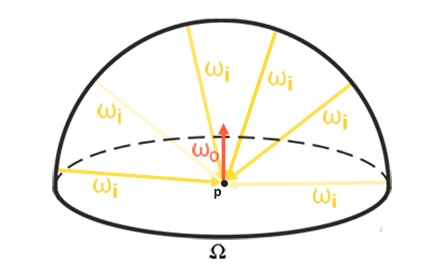
\includegraphics[scale=0.5]{hemisphere}}
  \caption{hemisphere}
\end{figure}

La ecuacion de render describe la radiancia de salida sobre un punto.
\begin{equation}
L_o(p, w_o) = \int_{\Omega} f_r(p, w_i, w_o)L_i(p, w_i)n\cdot{w_i}dw_i
\end{equation}

Siendo $\Omega$ la hemiesfera centrada en el punto sobre la que calculamos la irradiancia,
$f_r$ representa el brdf, $Li$, la irradiancia de la escena, mientras que $n\cdot{w_i}$ toma en
cuenta el \'angulo entre la de incidencia de la luz sobre la superficie.

\begin{equation}
L_o(p, w_o) = \int_{\Omega} (k_d + \frac{c}{\pi} + 
k_s \frac{DFG}{4(w_o\cdot{n})(w_i\cdot{n})})L_i(p, w_i)n\cdot{w_i}dw_i
\end{equation}

Los terminos $k_s$ y $k_d$ de la ecuacion de reflectancia son independientes, por lo que, de la
misma forma que en la iluminacion directa, los componentes se pueden separar en difuso y
especular.

\begin{equation}
L_o(p, w_o) = \int_{\Omega}
(k_d \frac{c}{\pi}) L_i(p, w_i)n\cdot{w_i}dw_i +
\int_{\Omega} 
k_s \frac{DFG}{4(w_o\cdot{n})(w_i\cdot{n})})L_i(p, w_i)n\cdot{w_i}dw_i
\end{equation}

La soluci\'on de la integral de la irradiancia de salida sobre $\Omega$ requiere samplear el entorno
en todas las direcciones posibles. Es por ello que en tiempo real, la soluci\'on consiste en
precomputar este c\'alculo y durante la ejecucion, calcular esta tabla de resultados.\\
ThreeJs utiliza dos enfoques, por una parte, mapas de irradiancia y por otra, light probes, que
utilizan spherical harmonics. Los mapas de irradiancia son una tecnica IBL (Image Based Lighting)
tratan todo el entorno como una fuente de luz y utilizan im\'agenes precomputadas que permiten
acelerar este calculo. Estas t\'ecnicas, aunque muy eficientes durante la ejecucion, son muy
costosas como para generarlas en tiempo real bajo demanda, la tecnica spherical harmonics, una
t\'ecnica que reduce el coste de generacion de los mapas de entorno a costa de comprimir la
informacion de irradiancia en un representacion frecuencias frente a espacio.

  \subsection{Componente difusa}
    La parte integral de la ecuaci\'on se resuelve utilizando el mapa de irradiancia,
    que utiliza un factor de corrci\'on en caso de estar modelando la refracci\'on interna,

    $$
    L_o(p, w_o) = k_d \frac{c}{\pi} \int_{\Omega}{L_i(p, w_i) n\cdot{w_i}dw_i}{}
    $$

    \begin{lstlisting}
float diffuseWrapFactor = 1.0;
#if defined(SUBSURFACE)
  diffuseWrapFactor *= saturate((dotNV + 0.5) / 2.25);
#endif

// Combine envmap and SH diffuse irradiance
vec3 Fd_SH = reflectedLight.indirectDiffuse * ( 1.0 - E ) * diffuseWrapFactor;
vec3 Fd_Lod = irradiance * BRDF_Diffuse_Lambert( material.diffuseColor )  * ( 1.0 - E ) * diffuseWrapFactor;
vec3 Fd = Fd_SH + Fd_Lod;

#if defined(SUBSURFACE)

  Fd *= saturate(subsurface + dotNV);

#endif
    \end{lstlisting}

  \subsection{Componente especular}
  \bgroup
    Para el especular, la tanto ThreeJs utilizan la t\'ecnica split-sum approximation
    \autocite{splitsum}. \'Esta t\'ecnica permite separar la en dos partes la soluci\'on de la
    integral.

    \begin{equation}
    L_o(p, w_o) =
    \int_{\Omega} k_s \frac{DFG}{4(w_o\cdot{n})(w_i\cdot{n})})L_i(p, w_i)n\cdot{w_i}dw_i = \\
    \int_{\Omega} k_s \frac{DFG}{4(w_o\cdot{n})(w_i\cdot{n})}) *
    \int_{\Omega}L_i(p, w_i)n\cdot{w_i}dw_i
    \end{equation}

    Por una parte, el mapa prefiltrado de entorno es un mapa preconvolucionado que tiene en cuenta
    los posibles valores de rugosidad del material de forma que a medida que el ruido es mayor, las
    reflexiones son de un color menos definido. Esta tecnica utiliza simplifica el calculo de
    la integral asumiendo la direccion de la vista igual a la direccion de sampleo.\\
    Por otra parte, el c\'alculo del BRDF se almacena en una textura, conocida como mapa de integral
    del BRDF, utilizando $n\cdot{w_i}$ en el eje $x$ y $roughness$ en el eje y.

    \begin{figure}[H]
      \vspace{0.5cm}
      \centering
        \frame{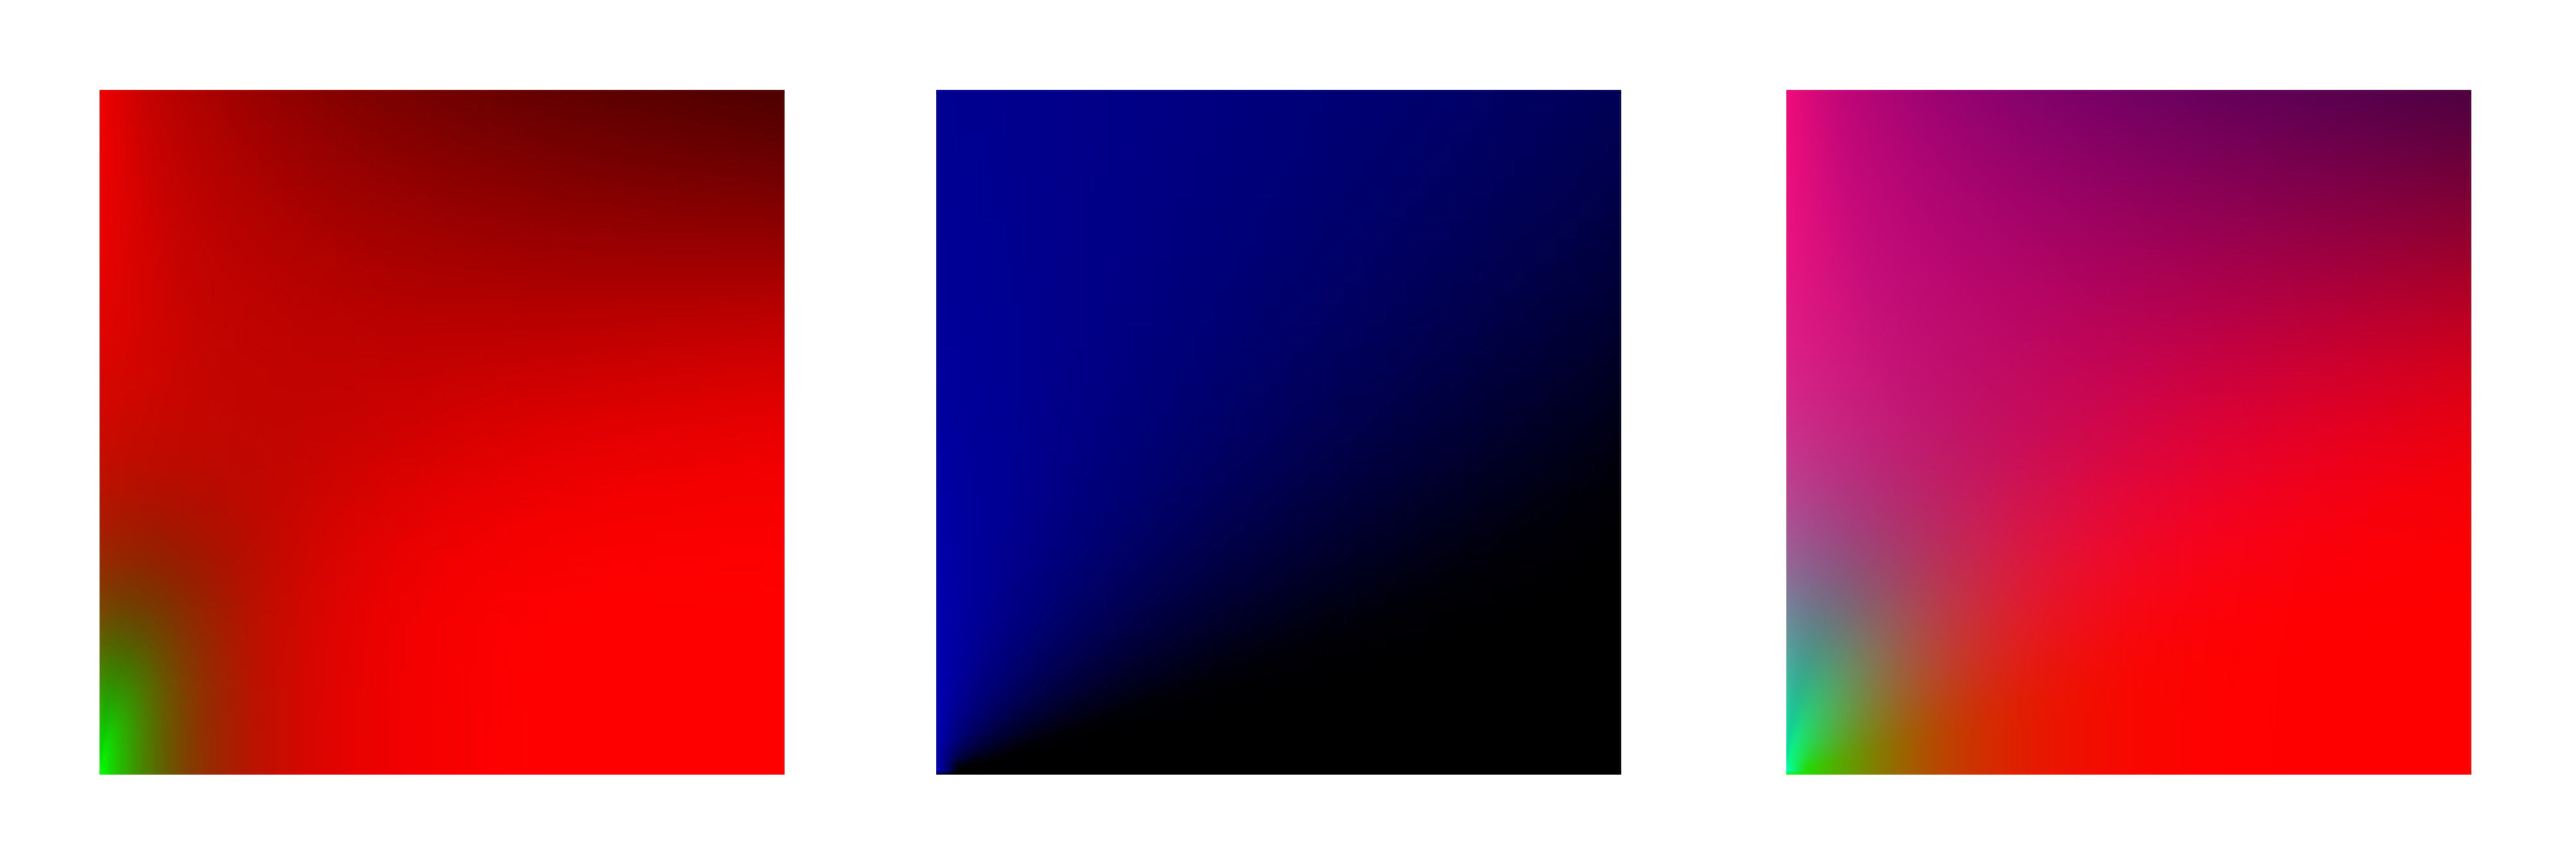
\includegraphics[scale=0.4]{splitsumcloth}}
      \caption{DFG tela}
    \end{figure}

    ThreeJs utiliza la aproximaci\'on anal\'itica para el c\'alculo de de mapa de integral del BRDF,
    la presentada por Epic Garmes \autocite{shadingmobile}, para aproximar el c\'alculo el BRDF GGX.

    \begin{lstlisting}[caption=Apromixaci\'on anal\'itica a la integral del BRDF en ThreeJs]
    vec2 integrateSpecularBRDF( const in float dotNV, const in float roughness ) {
      const vec4 c0 = vec4( - 1, - 0.0275, - 0.572, 0.022 );
      const vec4 c1 = vec4( 1, 0.0425, 1.04, - 0.04 );
      vec4 r = roughness * c0 + c1;
      float a004 = min( r.x * r.x, exp2( - 9.28 * dotNV ) ) * r.x + r.y;
      return vec2( -1.04, 1.04 ) * a004 + r.zw;
    }
    \end{lstlisting}

    Sin embargo, \'este c\'aculo no es v\'alido para nuestro BRDF, por que, deberemos utilizar una
    tabla en la que almacenar los resultados calculados para el BRDF presentado por Est\'evez y Kulla.
  \egroup
